\section{Smart Contracts}

A collection of smart contracts is used to efficiently manage the creation of the new event, the distribution of the tickets and also the registration of identities. Figure \ref{fig:smart-contract-overview} illustrates the architecture and their dependencies. The bold contracts are deployed only once whereas the \textit{EventContract} is newly deployed for every event. The library contains common stateless functionality across multiple contracts. The \textit{EventContract} inherits its functionality from the smart contract modules. These modules act as building blocks for creating contracts with different functionality. The contracts with a dotted outline add optional functionalities. This design pattern is chosen to reduce the deployment costs. It allows an event host to be specific on the functionality of the contract. For example as shown in the Figure \ref{code:smart-contract-inheritance}, it is possible to create an event without an aftermarket if the host desires to do so. 

\begin{figure}[H]
    \centering
    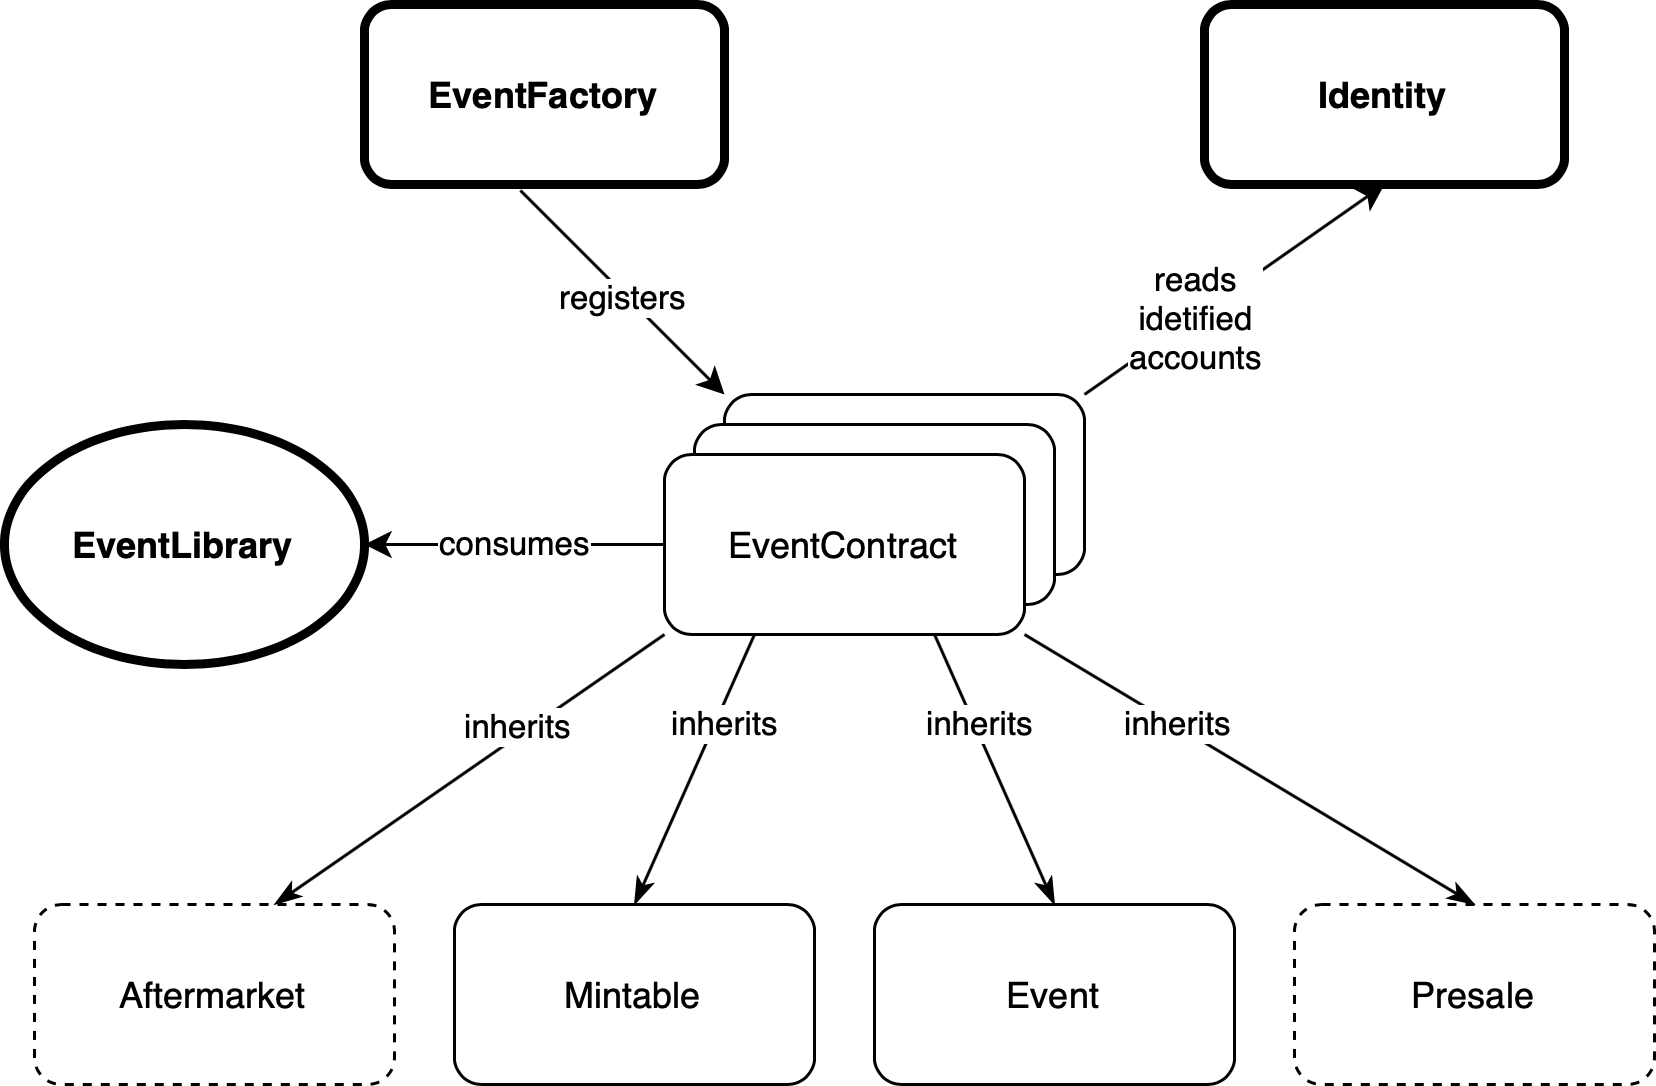
\includegraphics[width=14cm]{figures/smart-contract-overview-4.png}
    \caption{Smart Contract Overview}
    \label{fig:smart-contract-overview}
\end{figure}

\begin{figure}[H]
    \lstinputlisting[language=Solidity]{code-snippets/Inheritance.sol}
    \caption{Modular design pattern using inheritance}
    \label{code:smart-contract-inheritance}
\end{figure}

Each of the building blocks is described in more detail in the following sections.

\subsection{Event}
This building block is compulsory since it contains all the core functions and data structures that are used by the other contracts. 

The goal is to build a single contract for each event that manages the distribution and aftermarket of fungible as well as non-fungible tickets. The heart of the contract is the state that keeps track of the ownership of the tickets. For this a double mapping is used as shown in the Figure \ref{code:tickets} to to efficiently store and retrieve tickets from the contract.

\begin{figure}[H]
    \lstinputlisting[language=Solidity]{code-snippets/Tickets.sol}
    \caption{Tickets Mapping}
    \label{code:tickets}
\end{figure}


\subsection{Mintable}\label{sec:tickets}
The \textit{Mintable} contract is responsible for issuing new tickets. 

In order to differentiate between multiple ticket types, the following encoding schema was used for the ticket id. A ticket id is made up of three parts and is stored as a \textit{uint256} datatype. The first bit is the \textit{nf flag} which indicates if the ticket is fungible of non-fungible. If this bit is set, it is considered to be non-fungible otherwise fungible. 

The following 127 bits hold the ticket type and is incremented with every new type that is created. The type is used to store information that applies to all the tickets of that type. 

The last 128 bits are used for non-fungible tickets only. They store the id of a specific ticket. This is only relevant to non-fungible tickets since fungible tickets do not need an id as fungible tickets of the same type are indifferent to each other. 

As an example one can think of a seating area where each seat has an id. For such a scenario the \textit{nf} bit is set. The \textit{type} is set to the number \textit{4} in decimal (or \textit{100} in binary) since three other types have have been created before. The \textit{index} indicates the seat number. In this example the owner of this ticket has access to seat number 3 (or \textit{11} in binary).

\[
    uint256\ id = 
    \underbrace{1}_\text{nf flag (1 bit)}
    \underbrace{000...100}_\text{type (127 bit)}
    \underbrace{000...011}_\text{index (128 bit)}
 \]
 
With this encoding schema it is possible to store tickets of different types in the same mapping. Furthermore, using efficient shift operations and bitwise comparators the id can be decoded as shown in Figure \ref{code:tickets-decoding}.

\begin{figure}[H]
    \lstinputlisting[language=Solidity]{code-snippets/TicketsDecoding.sol}
    \caption{Tickets Decoding}
    \label{code:tickets-decoding}
\end{figure}

A similar encoding schema is also used for ERC1155 contracts \cite{erc1155}.

\subsection{Presale}\label{section:imp:presale}

To implement fair odds for the presale lottery, a user can only place one presale order for one ticket. The presale order will be placed in a list on the blockchain. Every new presale order will be appended to the list. Whenever the presale is over, and the lottery is triggered, a random number in the range of the number of presale orders is generated. The list of buy orders will then be cast to a ring by connecting the head with the tail. The winners of the lottery defined by the \textit{n} guests starting at the index in the ring that has been generated by the random number, where \textit{n} is the amount of tickets available. 

Figure \ref{fig:ring-lottery} shows an example where ten people signed up for the lottery but only five tickets are available. The random number evaluates to 7. The green boxes indicate the winners.

\begin{figure}[H]
    \centering
    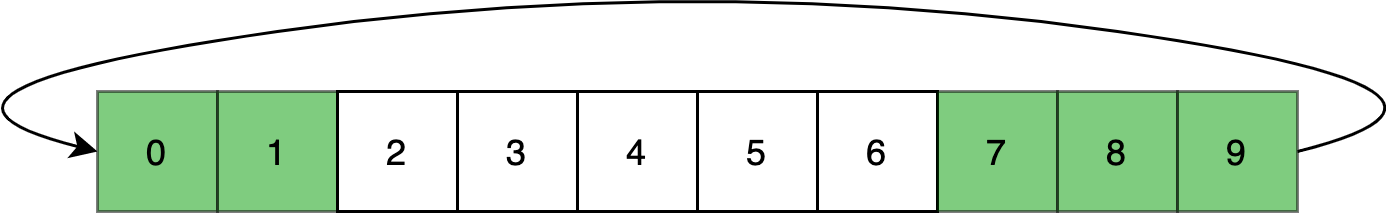
\includegraphics[width=14cm]{images/lottery.png}
    \caption{Ring Lottery Example}
    \label{fig:ring-lottery}
\end{figure}

This ensures fair odds for everybody and also lets people that want to attend an event together maximize the chance that both win the lottery, by placing their presale order at the same time and therefore try to get a place in the list next to each other.

\subsection{Aftermarket}
This optional building block adds the functionality of a decentralized exchange. It implements the queuing architecture as described in Section \ref{section:aftermarket}. A queue is constructed of two structs as show in Figure \ref{code:queue}. The members \textit{head} and \textit{tail} act as pointers to efficiently perform operations on the queue such as \textit{pop} and \textit{enqueue}. This data structure is used for the buying and the selling queue. 

\begin{figure}[H]
    \lstinputlisting[language=Solidity]{code-snippets/Queue.sol}
    \caption{Queue in a solidity contract}
    \label{code:queue}
\end{figure}

If a user wants to withdraw from a queue, he must provide his position in the queue to efficiently perform this task without the need of looping over the entire queue. This index is emitted as a Solildity event when a user is enqueued. 

\subsection{Library}
A library in Solidity allows to deploy common functionality that does access the state of the contracts. For example, the functions shown in Figure \ref{code:tickets-decoding} are all deployed as part of a library. But also error messages and other constants are outsourced to the library. This helps in managing code consistency and reduces redundancy.

\subsection{Identity}
This building block is essential to achieve the goal of eliminating an aftermarket run by scalpers. The identity contract is used to store identity proofs to the blockchain. An off-chain service checks the guest's identity. The proof of the identity is then stored using a double mapping of an ethereum address to an ethereum address to an integer. This integer is describing the level of identity an Ethereum address has had approved with a given identity provider. 

In order for an identity approver to be able to save identity proofs for other guests to the blockchain, he has to register as an identity approver first. To do this, the approver provides some information about the levels he is using. This information is saved to IPFS. The IPFS hash is then saved to the blockchain to register the approver.

\subsection{Economics}\label{sc:econom}
Paying all involved stakeholders in a transparent matter is necessary. Thus, the smart contract allows to pass affiliate addresses and GUI builders as arguments for methods such as buying a fungible ticket (Figure \ref{code:buy-ticket-function}). A GUI builder can hardcode his Ethereum address in the frontend application and receives a cut for every ticket sold on his application. 

Besides the GUI provider's address, an additional affiliate address can be passed in the argument. Affiliates are marketing companies or influential people that advertise the venue to the event guests and redirect them to a GUI providers. It is important to note that the affiliate has to trust the GUI provider that he includes the affiliate's address in the smart contract call. However, with the proposed design it is also in the GUI provider's interest that other entities redirect guests to their platform. Furthermore, with the open nature of the design, there is no lock-in effect with any of the GUI providers and they can be replaced if they do not act trustworthy.

The identity providers always receives a fraction of the ticket price as shown in Figure \ref{code:buy-ticket-function} on line 22.

\begin{figure}[H]
    \lstinputlisting[language=Solidity]{code-snippets/BuyTicketFunction.sol}
    \caption{Buying fungible tickets with affiliate addresses}
    \label{code:buy-ticket-function}
\end{figure}



